\subsection{Topological Preference in Path-Planning}

% add outline page with current section highlighted.
\begin{frame}{Outline}{ $ \null $ }
	%\tableofcontents[currentsection]
	\tableofcontents[currentsection,currentsubsection]
\end{frame}

\begin{frame}{Interactive Path-Planning}{Related Work}

\begin{columns}
\column{0.47\textwidth}
\begin{figure}
	\centering
	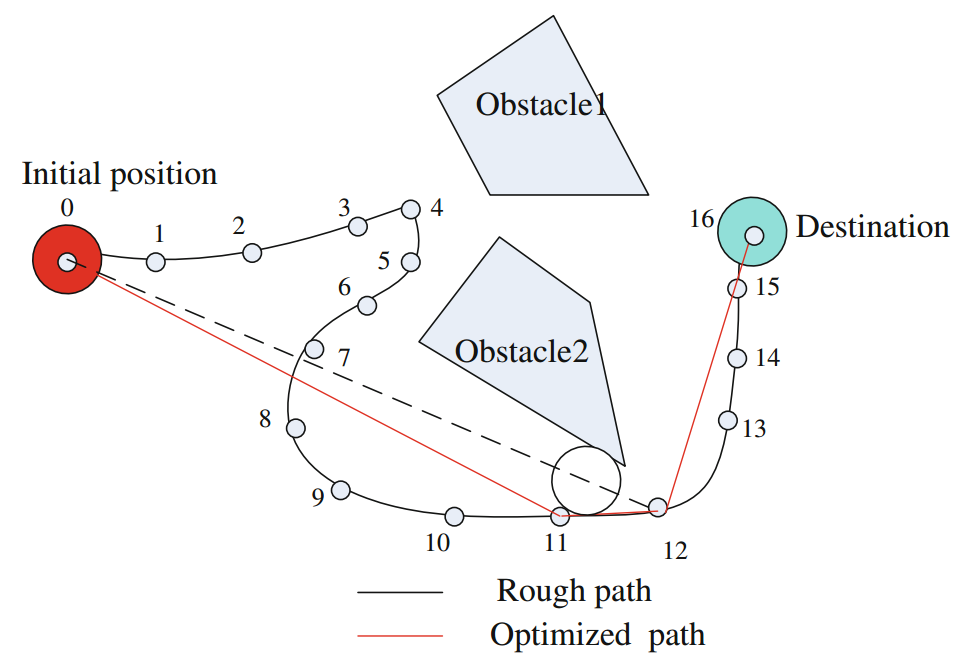
\includegraphics[width=.9\linewidth]{figure/interactive_path_planning}
	\caption{\tiny {\it Chen et al.} ``Haptic-based interactive path planning for a virtual robot arm.'' International Journal on Interactive Design and Manufacturing 2010.}
\end{figure}

\column{0.47\textwidth}
\begin{itemize}
\item A human initializes a rough path
\item The path is optimized by node manipulation
\item The node manipulation is driven by the potential fields
\end{itemize}

\end{columns}


\end{frame}

\begin{frame}{Reference Path}{Related Work}

\begin{columns}
\column{0.67\textwidth}
\begin{figure}
	\centering
	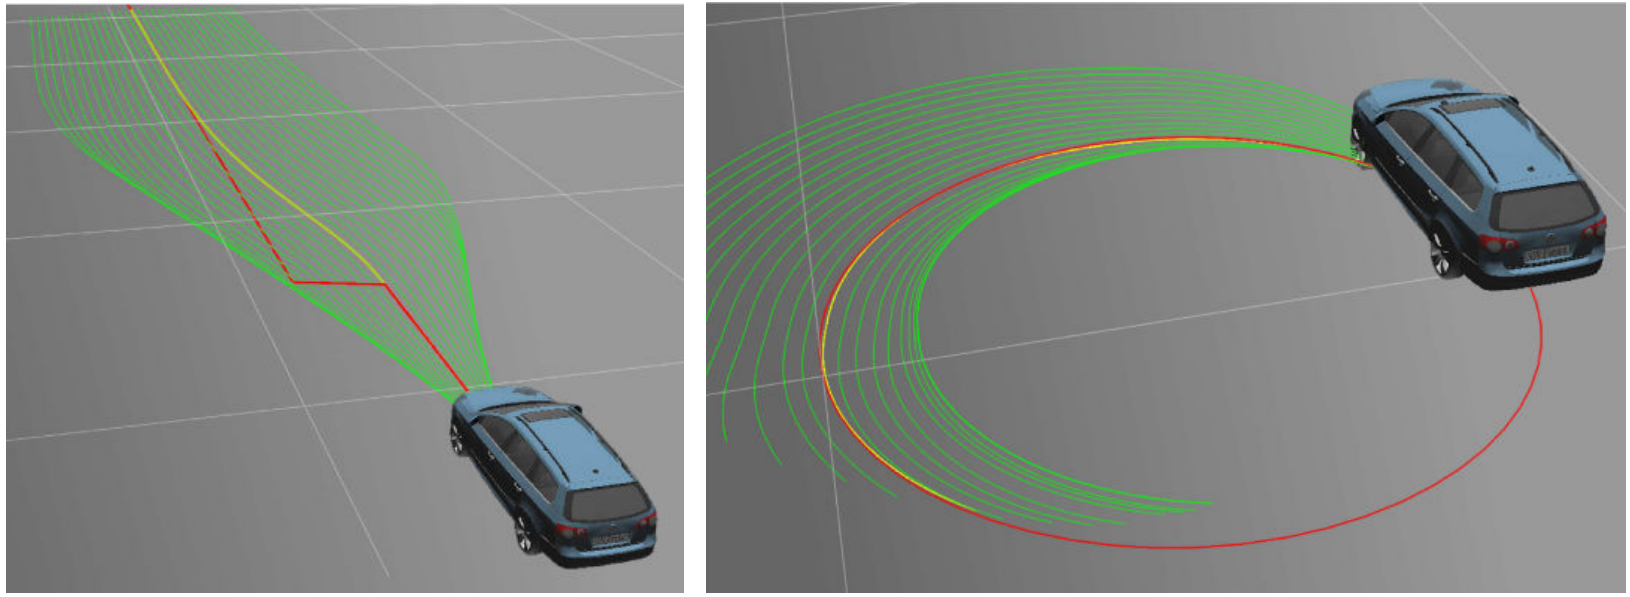
\includegraphics[width=\linewidth]{figure/interactive_path_planning2}
	\caption{\tiny {\it Schwesinger et al.} ``A sampling-based partial motion planning framework for system-compliant navigation along a reference path.'' IEEE Intelligent Vehicles Symposium (IV) 2013.}
\end{figure}

\column{0.32\textwidth}
\begin{itemize}
\item (Red) Reference path
\item (Green) Solution path set
\item (Yellow) Optimal path
\end{itemize}

\end{columns}

\end{frame}

\begin{frame}{Homotopy}{Related Work}

\begin{block}{Definition}
Given two paths, if one can be deformed into the other without encroaching any obstacle, they are said to be {\bf homotopic}.\footnotemark
\end{block}

\begin{columns}
\column{0.47\textwidth}
\begin{figure}
	\centering
	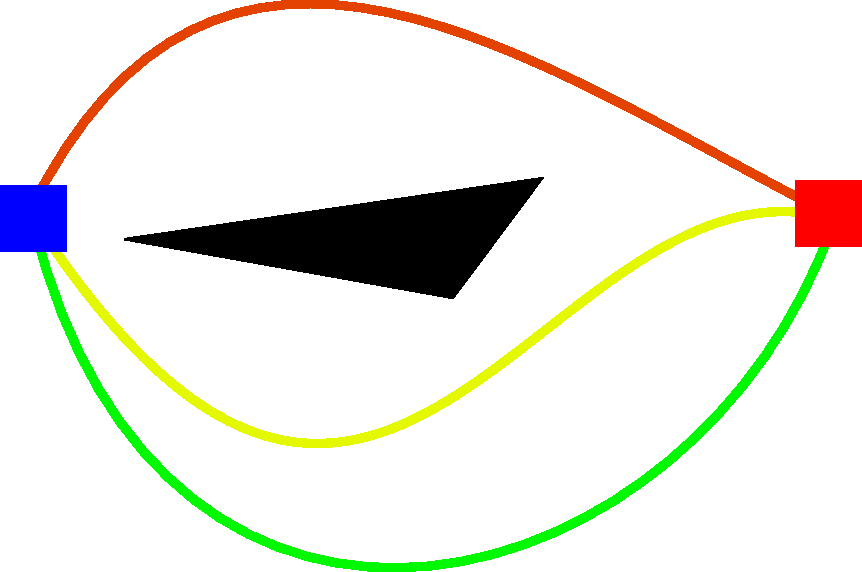
\includegraphics[width=.8\linewidth]{figure/path_homotopy}
\end{figure}

\column{0.47\textwidth}
\begin{figure}
	\centering
	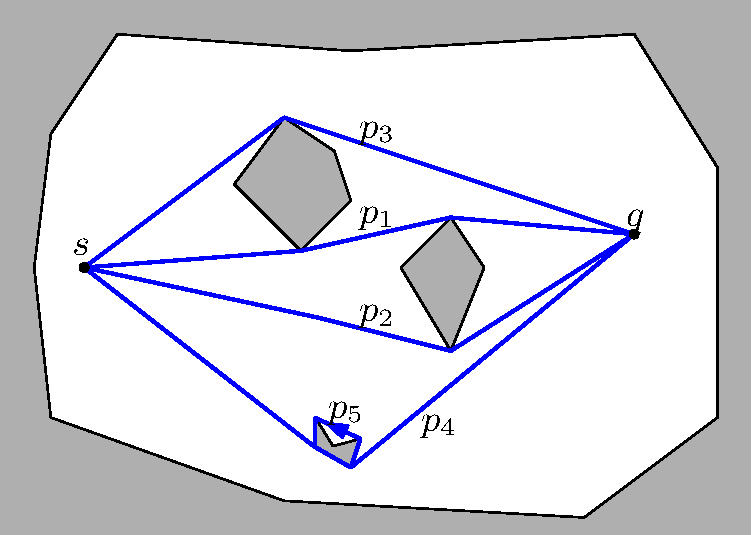
\includegraphics[width=.8\linewidth]{figure/path_homotopy_map}
	\caption{\tiny http://www.cs.helsinki.fi/group/compgeom/ksp/}
\end{figure}

\end{columns}

\begin{block}{}
	{\bf Homotopy class} is the set of paths that are all homotopic to each other
\end{block}

\footnotetext[1]{\tiny {\it Hernandez et al.} ``A comparison of homotopic path planning algorithms for robotic applications.'' Robotics and Autonomous Systems 2015.}

\end{frame}

\begin{frame}{Voronoi-based Homotopy Identification}{Related Work}

\begin{columns}

\column{0.55\textwidth}
\begin{figure}
\begin{subfigure}
	\centering
	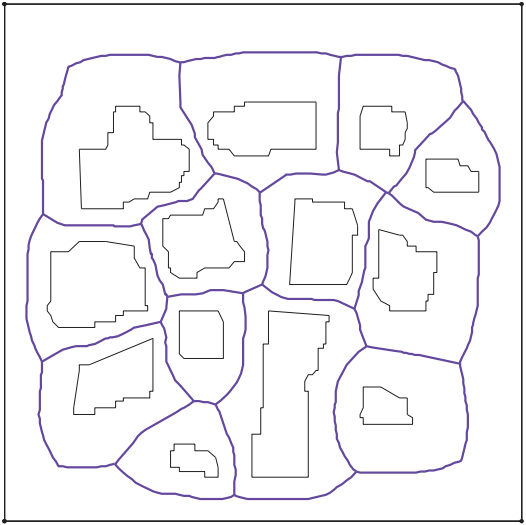
\includegraphics[width=.49\linewidth]{figure/voronoi_homotopy1}
\end{subfigure}
\begin{subfigure}
	\centering
	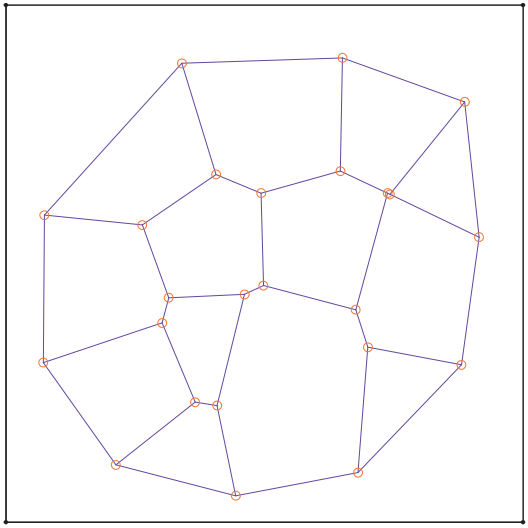
\includegraphics[width=.49\linewidth]{figure/voronoi_homotopy2}
\end{subfigure}
\\
\begin{subfigure}
	\centering
	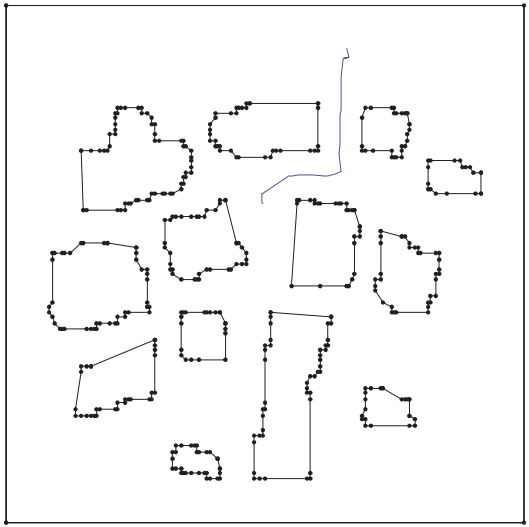
\includegraphics[width=.49\linewidth]{figure/voronoi_homotopy3}
\end{subfigure}
\begin{subfigure}
	\centering
	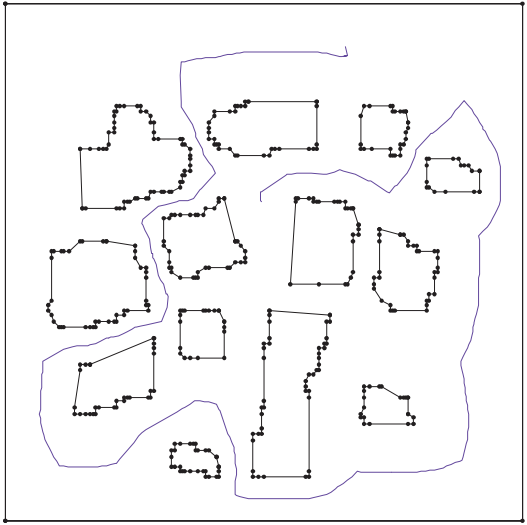
\includegraphics[width=.49\linewidth]{figure/voronoi_homotopy4}
\end{subfigure}
\end{figure}

\column{0.42\textwidth}
\begin{block}{}
\begin{itemize}
\item Voronoi diagram
\item Simplified graph
\item A non-simple path not reported 
\item A simple path in the same homotopy class
\end{itemize}
\end{block}

\end{columns}

\tiny{ {\it Banerjee et al.} ``A framework of Voronoi diagram for planning multiple paths in free space.'' Journal of Experimental \& Theoretical Artificial Intelligence 2013.}

\end{frame}

\begin{frame}{Complex-Integral-based Homotopy Identification}{Related Work}

{\bf Cauchy Integral Theorem} ``If two different paths connect the same two points, and a function is holomorphic everywhere "in between" the two paths, then the two path integrals of the function will be the same.'' [Wikipedia]

\begin{columns}
\column{0.5\textwidth}
\begin{figure}
\begin{subfigure}
	\centering
	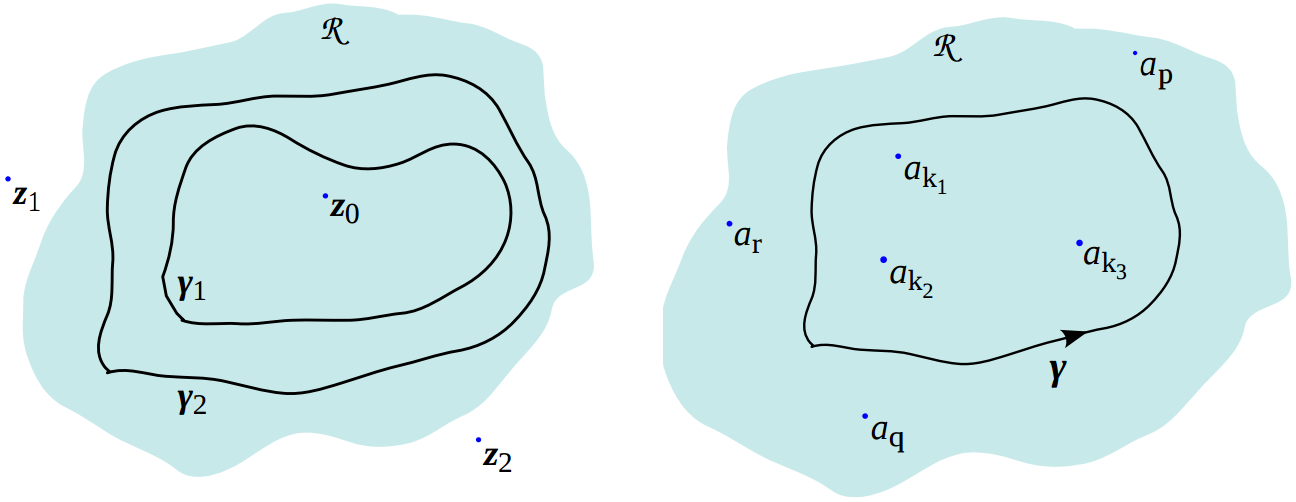
\includegraphics[width=\linewidth]{figure/cauchy_theorem}
\end{subfigure}
\\
\begin{subfigure}
	\centering
	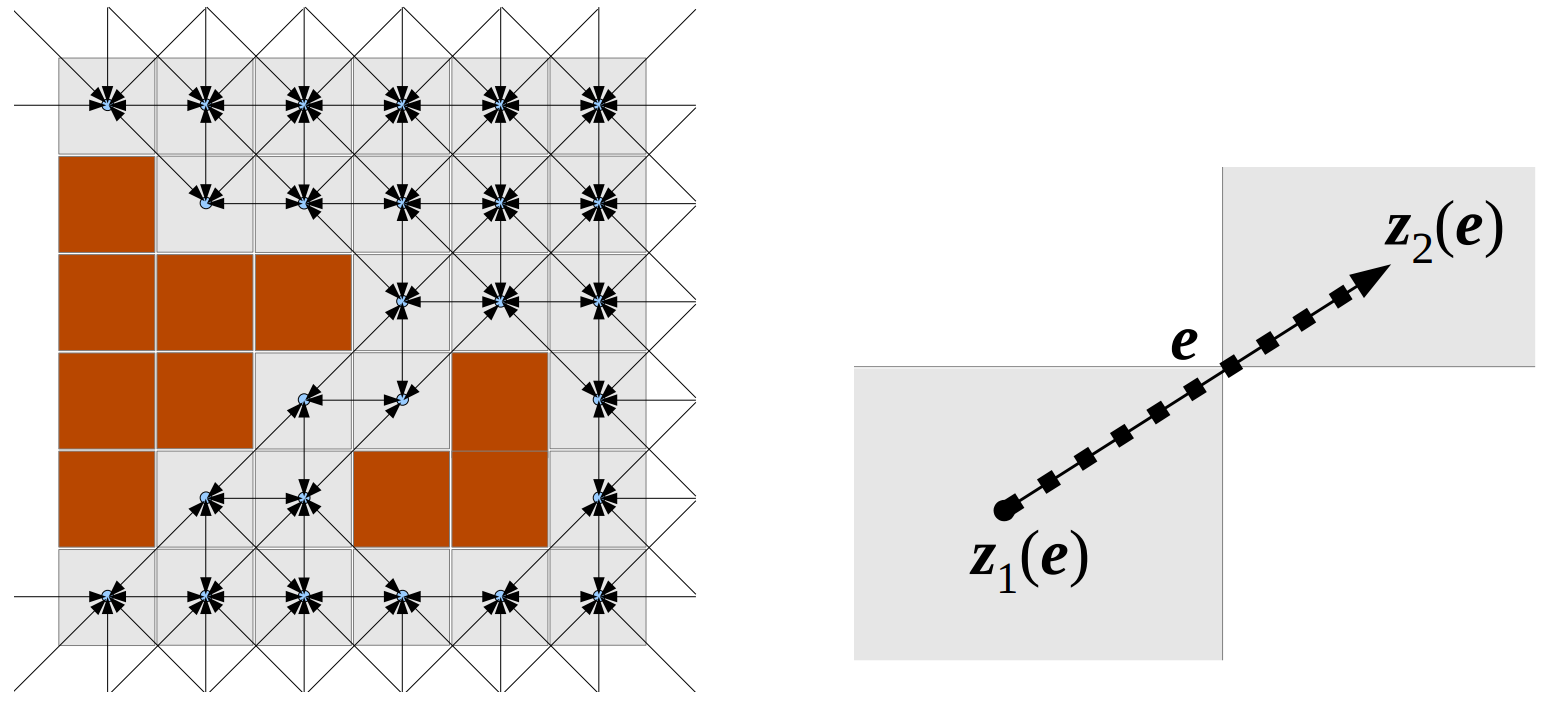
\includegraphics[width=\linewidth]{figure/cauchy_theorem2}
\end{subfigure}
\end{figure}

\column{0.49\textwidth}
\begin{block}{}
\begin{itemize}
\item Complex plane
\item Undefined point in obstacle
\item Cauchy Theorem
\end{itemize}
\end{block}

\begin{block}{}
\begin{itemize}
	\item Map discretization
	\item Complex integral of each segment
\end{itemize}
\end{block}
\end{columns}

\tiny{ {\it Bhattacharya et al.} ``Search-based path planning with homotopy class constraints.'' AAAI 2010. }

\end{frame}

\begin{frame}{Homotopic RRT}{Related Work}

\begin{columns}

\column{0.47\textwidth}
\begin{figure}
	\centering
	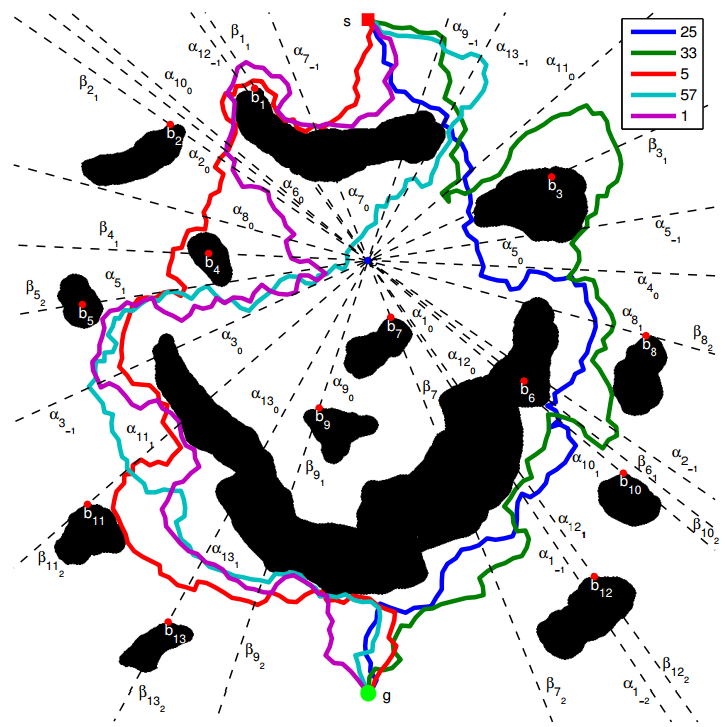
\includegraphics[width=\linewidth]{figure/homotopic_rrt}
	\caption{\tiny {\it Hernández et al.} ``A topologically guided path planner for an auv using homotopy classes.'' IEEE International Conference on Robotics and Automation (ICRA) 2011.}
\end{figure}

\column{0.47\textwidth}
\begin{block}{}
\begin{itemize}
\item Reference frames
\item Convert paths into strings
\item Using RRT to find paths
\end{itemize}
\end{block}

\begin{block}{}
	\begin{itemize}
		\item Cannot identify all the homotopic equivalence
	\end{itemize}
\end{block}
\end{columns}

\end{frame}

\begin{comment}
\begin{frame}{Funnel Algorithm}{Related Work}

\begin{columns}

\column{0.4\textwidth}
\begin{figure}
	\centering
	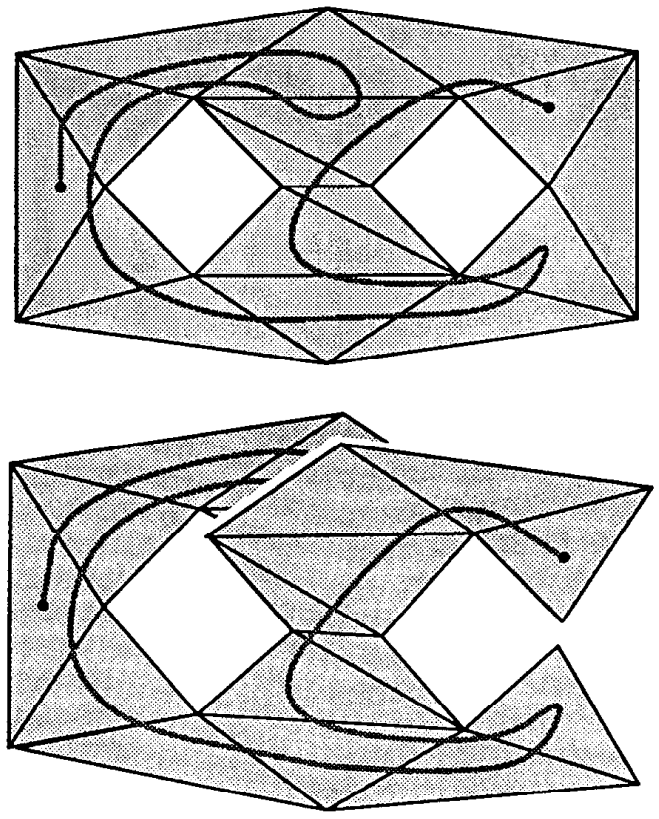
\includegraphics[width=\linewidth]{figure/funnel_algorithm}
\end{figure}

\column{0.57\textwidth}

\end{columns}

\tiny{ {\it Hershberger et al.} ``Computing minimum length paths of a given homotopy class.'' Computational geometry 1994. }

\end{frame}
\end{comment}
